\documentclass[14pt, a4paper]{extreport}
\usepackage{titlesec}
\usepackage{graphicx}
\usepackage{amsmath}
\usepackage{mathtools}
%\usepackage{newtxtext,newtxmath}
\usepackage{hyperref}
\hypersetup{
	colorlinks=true,
	urlcolor=red,
	linkcolor=red,
}
\usepackage{tocbibind}
\usepackage{wrapfig}
\usepackage{float}
\title{Probabilistic Trip estimation}
\author{Jaydeep Nandi, Kalyan Koripella, Shishir Thakur, Lakhan Lal}

\pagenumbering{roman}
\begin{document}

	
	\maketitle
	\titleformat{\chapter}[display]{\normalfont\bfseries}{}{0pt}{\Large}
	\setcounter{page}{1}
	\tableofcontents
	\chapter[Declaration]{Declaration}
	\setcounter{page}{1}
	
	\newpage
	\chapter[Certificate from HOD]{Certificate From HOD}
	\chapter[Certificate from Supervisor]{Certificate From Supervisor}		
	\chapter[Acknowledgements]{Acknowledgements}
	\chapter[Abstract]{Abstract}
	\newpage
	\pagenumbering{arabic}
	
	
	\chapter[Introduction]{Introduction}
	\setcounter{page}{1}
\section[Voltage sag]{Voltage sag}
\paragraph{}
Voltage sag is one of the most significant power quality sues that can affect the majority of sensitive equipments like personal computers (PC), adjustable speed drives (ASD), programmable logic controllers (PLC). Voltage sag is defined as a decrease in rms voltage or current at the power frequency for durations of 0.5 cycle to 1 min. Typical values are from 0.1 to 0.9 pu.[IEEE Recommended Practice for Evaluating Electric Power System Compatibility With Electronic Process Equipment]. Voltage sags are present in power systems, but only during the past decades customers are becoming more sensitive to the inconvenience caused [Pirjo Heine and Matti Lehtonen, “Voltage sag distributions caused by power systems faults,” IEEE Transactions on Power Systems, vol.18, No.4, pp.1367-1373, November 2003]. Voltage sag can cause serious problems to sensitive loads, because these loads often drop off-line due to voltage sag. Out of the various disturbances that effect the power quality, voltage sag happens to be the most frequent disturbance. If a voltage sag occurs for a longer duration it is called an undervoltage. 
\paragraph{}
\textbf{Characteristics of Voltage sags:}
\begin{enumerate}
    \item 	\textbf{Magnitude}:- The minimum value of Vrms(1/2) recorded during a voltage sag. The magnitude is expressed as a value in volts or as a percentage or per-unit value of the declared voltage or sliding-reference voltage.[ IEEE Guide for Voltage Sag Indices]
    
    \item 	\textbf{Duration}:- The voltage sag duration is nothing but the period of time in which the voltage is lower than the stated limit; normally sag duration is less than 1 second [IEEE Std. 493, 1997]. The voltage sag starts when at least one of the rms voltages drops below the sag-starting threshold. The sag ends when all three voltages have recovered above the sag-ending threshold.
    
    \item \textbf{Unbalance of sag}:- In the power system the faults are classified as symmetrical (balanced) and unsymmetrical (unbalanced) depending on the type of fault. If three phase fault occurs, the sag will be symmetrical but if the fault is single phase, double phase or double phase to ground faults the sag in three phases will not be symmetrical.
    
    \item 	Point on wave of sag initiation.
    
\end{enumerate}

\textbf{Types of Voltage Sag:}
\begin{enumerate}
    \item \textbf{Single phase sags}:- These are frequently occurring voltage sags and are basically due to the phase to ground faults.
    
    \item \textbf{Phase to phase sags:} The two phase or phase to phase sags are caused by tree branches, adverse weather, animals or vehicle collision with utility poles.
    \item \textbf{Three phase sags:} - These sags are caused by switching or tripping of a 3 phase circuit breaker.These sags are caused by switching or tripping of a 3 phase circuit breaker, switch or recloser which will create three phase voltage sag on other lines fed from the same substation.
    
    
\end{enumerate}

\textbf{Following are some of the causes for the occurrence of voltage sag:-}\begin{enumerate}
    \item Starting of motors can cause a voltage sag as a large amount of current will be drawn during starting when compared to current drawn while running at rated speed.
    
    \item Excessive or sudden load changes can cause a voltage sag.
    
    \item 	When a fault occurs there will be voltage sag until the protective switch gear operates.
\end{enumerate}

\section[Voltage Tolerance Curves]{Voltage Tolerance Curves}
\subsection{Automatic Speed Drives:} An ac ASD controls the speed of an induction or synchronous motor by converting fixed frequency/fixed magnitude ac mains supply voltage to a variable frequency/variable magnitude voltage at the motor terminals.  The ASDs are three-phase equipment and d ifferent combinations of three phase voltages during the sags have different effects on their operation. Testing of ASDs was conducted with the following three types of voltage sags:

\begin{enumerate}
    \item Three-phase balanced voltage sags.
    \item Generalized two phase voltage sag.
    \item Generalized single phase voltage sag.
\end{enumerate}

 To illustrate this, the test procedure used with rectangular voltage sags is described: 
 
 \begin{enumerate}
     \item The drive was first connected to the voltage sag generator (VSG) which supplies the drive with rated input characteristics. Controlled motor was started unloaded.
     
     \item The motor was loaded with one of three load types and the selected torque. The speed of the motor was adjusted to one of the pre-selected values. One of three voltage sag types was selected for testing. The point on wave of the sag initiation and phase shift during the sag were set.
     
     \item Voltage sags were applied in steps of 1\% of rated value, starting from 0 V. For each sag magnitude, the duration of
the sag was prolonged until some of drive protection systems activate the disconnection of the drive, or, if there is no disconnection, up to a few seconds. The critical sag duration was ascertained by up to 10 repeated measurements. A 5–10 s recovery time was allocated between the consecutive voltage sags.

\item In testing with sags for which voltage in the unsagged phase(s) was used as a parameter, this value was changed in 10\% steps from 0–100\% of the rated value, and measurements described in step 3 were repeated.

\item The point onwave of voltage sag initiation was adjusted in steps of $15^{o}$ (from 0 to $360^{o}$) and measurements described in step 3 were repeated.

\item The phase shift during the sag was changed in steps of 15 (from 0 to ±$90^{o}$) and measurements described in step 3 were repeated. 

\item The speed of the motor was changed to the next value and measurements described in step 3 were repeated (motor speeds selected for testing were: 100, 75, 50, and 25\% of rated motor speed).

\item Loading torque was changed to the next value, and measurements described in step 3 were repeated. Torque values selected for testing were: 100, 75, 50, 25, and 0\% of rated motor torque.

\item The load typewas changed to next of three types (i.e., constant torque load, load with linear relationship between the speed and torque, and load with quadratic relationship between the speed and torque) and measurements described in step 3 were repeated.

\item The voltage sag type was changed to the next of the three types and measurements described in step 3 were repeated.


 \end{enumerate}
 
 \begin{figure}
     \centering
     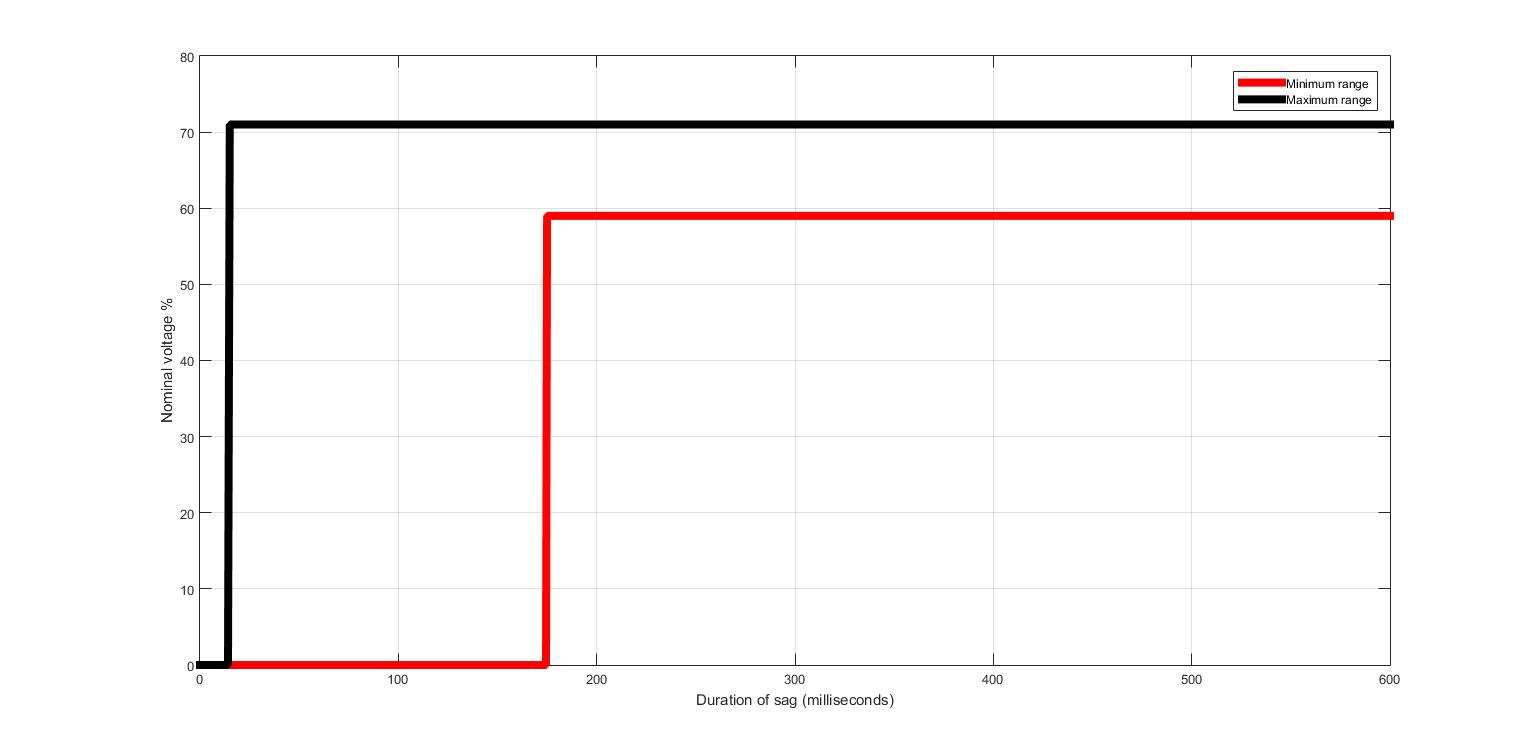
\includegraphics[width = \textwidth]{asd2.jpg}
     \caption{Single graph representation of drive sensitivity to various types of voltage sags}
     \label{fig:asd_characteristics}
 \end{figure}

\subsection{Personal computers (PCs)} Personal computer (PC) is a a general-purpose, rather complex electronic computing device designed to be operated by one person at a time. PCs can be implemented as “real-time” systems (i.e., for real-time control of various external devices), for online control of communication between two or more locations, or as a part of continuous process-control applications. Two software malfunction criteria that may result in different voltage-tolerance curves for PCs were considered in the tests: a) lockup of a read/write operation, and b) blockage of the operating system (OS). Tests were performed with rectangular voltage sags and an ideal voltage supply, as well as with nonrectangular sags occurring during the start of the large motors. The following procedure was used in tests with rectangular voltage sags.

\begin{enumerate}
    \item The computer (with all input/output (I/O) and pointing devices connected) was switched on and allowed to boot and load the operating system.
    
    \item Read/write operation (copying of different files from CD-ROM to the computer’s hard drive) was initiated.
    
    \item Voltage sags were applied in steps of 1\% of rated voltage, starting from 0 V. The point on wave of the sag initiation and the phase shift during the sag were both kept constant. For each voltage sag magnitude, the duration of the sag was progressively increased until lockup of copying operation was obtained, or the operating system was blocked, or the computer was forced to restart, or if none of the former happened up to a few seconds. The critical sag duration for each of these hardware/software criteria was ascertained by up to ten repeated measurements for each value of the sag magnitude. In cases when the tested computer had different sensitivities to voltage sags with respect to different software/hardware criteria, it would first lock up the read/write operation, then it would block the OS, and, finally, it would restart. A recovery time of 5-10 s was allocated between the consecutive voltage sags.
    
    \item The point on wave of voltage sag initiation was adjusted in steps of $15^{o}$ (from 0 to $360^{o}$) and the  measurements described in Step 2 were repeated.
 \item  The phase shift during the sag was changed in steps of 15 (from 0 to $90^{o}$ ) and the measurements described in Step 3 were repeated.
 \end{enumerate}
 \begin{figure}
     \centering
     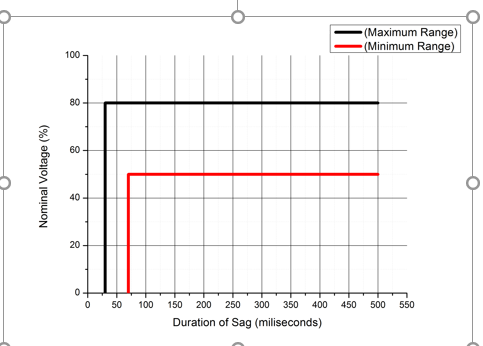
\includegraphics[width=\textwidth]{pc.PNG}
     \caption{ Voltage tolerance curve for Personal Computer}
     \label{fig:PC_characteristics}
 \end{figure}
 
 \subsection{AC Coil Contactors:} Switching elements are necessary for efficient control, isolation, protection, and signaling in all electrical systems. Out of all the other switching elements contactors make possible the centralized or remote control of motors and other industrial machinery. They can be integrated easily with other important circuits to perform more complex functions such as coordinated protection, time-dependent operation, or factory automation. Contactors are designed to disconnect the load or circuit they control when the main power supply (control voltage) is interrupted. While testing AC Coil Contactors. Tests were performed with rectangular voltage, an ideal voltage supply, and also with two-stage sags and with sags due to the starting of large motor. The testing of the contactors was always conducted according to a well-defined procedure. For example, the procedure for testing with rectangular voltage sags proceeds as follows.
 \begin{enumerate}
     \item The contactor’s main electrical contacts are engaged by applying nominal voltage to the ac coil terminals (by pressing
the “ON” button).
\item Keeping constant the values of the point on wave of sag initiation and phase shift during the sag, voltage sags are applied in steps of 1\% of nominal voltage, starting from 0 V. For each voltage sag magnitude, the duration of the sag is progressively increased until contactor disengages, or up to a few seconds. The sag duration required for disengagement is ascertained by ten repeated measurements for each sag magnitude, point on wave of initiation and phase shift. After each disengagement, a minimum of 5-s recovery time is allocated before the next voltage sag is applied. 
\item The point on wave of voltage sag initiation is adjusted in steps of $15^{o}$ (from 0 to $360^{o}$) and the measurements described
in step 2 are repeated.
\item The phase shift during the sag is changed in steps of $15^{o}$ (from 0 to $90^{o}$) and the measurements described in step 2 are
repeated. 
\end{enumerate}
 \begin{figure}
     \centering
     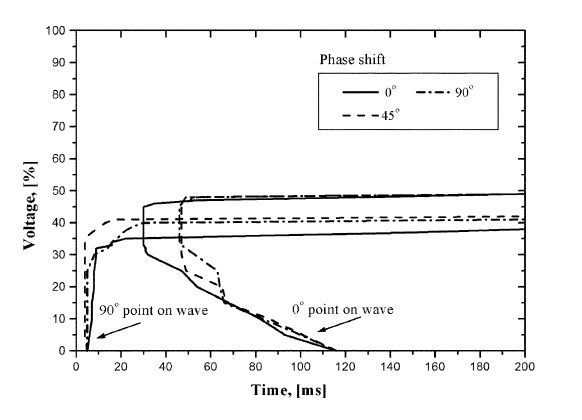
\includegraphics[width=\textwidth]{contactor.png}
     \caption{Contactor Characteristics}
     \label{fig:contactor_characteristics}
 \end{figure}
 \subsection{Programmable Logic Controller (PLCs) } PLCs (Programmable Controllers) have been utilized widely as the automation backbone of industrial process sectors such as mechanical manufacturing, coal mine, chemical industry, power engineering and so on[ Chen Zhuo “Exploring the Application of Programmable Logic Controller (PLC) [J]” Electronics Word, no. 23, pp. 174-177, Dec., 2015]. This is an important category of equipment for industrial processes because the entire process is often under the control of these devices. The sensitivity to voltage sags varies greatly but portions of an overall PLC system have been found to be very sensitive. 
 
 \begin{figure}
     \centering
     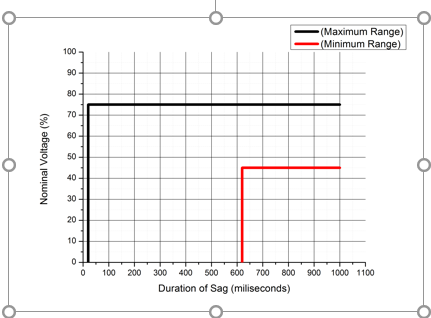
\includegraphics[width=\textwidth]{plc.PNG}
     \caption{Voltage tolerance curve for PLC}
     \label{fig:my_label}
 \end{figure}
 
 \subsection{5 HP AC Drive} This AC drive controls the speed of an induction or synchronous motor by converting fixed frequency/fixed magnitude ac mains supply voltage to a variable frequency/variable magnitude voltage at the motor terminals. Testing of 5 HP AC Drive is similar to the testing of ASD. After performing the tests we get the voltage tolerance curve of the 5 HP AC Drive
 \begin{figure}
     \centering
     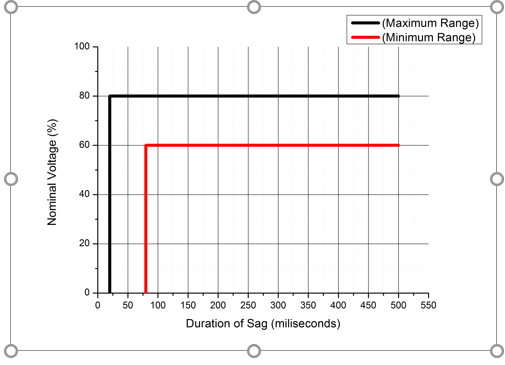
\includegraphics[width=\textwidth]{5hpacdrive.PNG}
     \caption{Voltage tolerance curve for 5 HP Ac Drive}
     \label{fig:5hp_ac_drive}
 \end{figure}
 \subsection{Motor Starter}The voltage tolerance curves for the motor starter after performing the tests is attached \ref{fig:motor_starter}.
 \begin{figure}
     \centering
     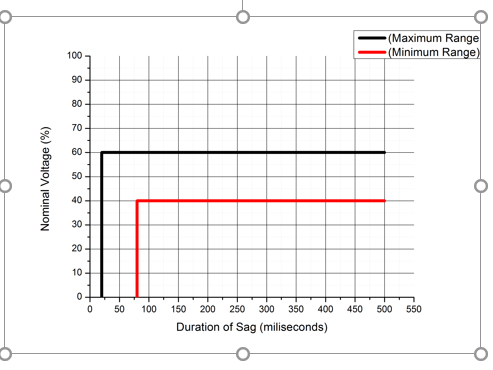
\includegraphics[width=\textwidth]{motorstarter.PNG}
     \caption{Motor Starter}
     \label{fig:motor_starter}
 \end{figure}

		\chapter[Literature Review]{Literature Review}
			\begin{enumerate}
\item 
    \begin{enumerate}
        \item{\textbf{Name of the chapter:}} Impersonal probability assessment of equipment trip due to voltage sag. 

       \item{\textbf{Name of the author:}}Ying Wang, Yong Huang,Chao, Xianyong Xiao,college of electrical engineering. \linebreak
        
         \item{\textbf{Journal:}}2010, IEEE
        \item{\textbf{Summary:}}The paper has provided
an objective method,
using maximum entropy
principle to determine the
stochastic distribution of
any random event in
mathematical field, which
is a good alternative to
solve the probability
model of voltage tolerate
curve for given sensitive
equipment. As a case
study PC is simulated
under different conditions
and compared with the
traditional methods by
Monte Carlo.
\end{enumerate}
        
        \item 
        
        \begin{enumerate}
            
        \item{\textbf{Name of the chapter:}}A voltage sag
index
considering
compatibility
between
equipment and
supply
\item{\textbf{Name of the author:}}Cheng- Chieh
Shen, student
member, IEEE
Chan-Nan Lu,
senior member,
IEEE
\item{\textbf{Journal:}}IEEE
transactions
on power
delivery, Vol
22, No.2,
April 2007
\item{\textbf{Summary:}}This paper presents a
voltage sag index which
would be very useful for
indicating system
performance experience at
different locations. Fuzzy
logic techniques are
applied to quantify
voltage sag disturbance
level where retained
magnitude and sag
duration are the inputs to
the proposed system and
the output is an index
that indicated relative
severity of the
\end{enumerate}
\item \begin{enumerate}
\item{\textbf{Name of the chapter:}}Assessment of
financial losses
due to voltage
sag in an Indian
distribution
system
\item{\textbf{Name of the author:}}A.K Goswami,
student
member, IEEE
C P Gupta,
member, IEEE
G K Singh,
Department of
electrical
engineering,
IIT Roorkee
\item{\textbf{Journal:}}2008 IEEE
Region 10
colloquium
and the third
international
conference on
Industrial and
information
systems,
Kharagpur,
India,
December
2008
\item{\textbf{Summary:}}This paper presents a
practical implementation
of the stochastic
assessment of annual
financial losses due to
voltage sags considering
the uncertainties involved
with sensitivity and
interconnection of
equipments in individual
process, customer types
and location of the
process in system
network. The evaluation
of the impact of the
voltage sags at a
particular site in a
network involves two
basic steps – voltage sag
assessment and economic
assessment. The fault
positons method is used
for the stochastic
prediction of voltage sag
and for economic
assessment of customer
losses due to voltage sags,
it is assumed that every
nuisance trip of an
industrial process requires
24 hours of restoration
time. (Any other duration
adopted would not affect
the methodology used)The damage costs
reported by various
categories of customers
for 24 hours long
interruption are taken as
the damage costs for
process trips due to
voltage sags.

    \end{enumerate}
    
    \item
    \begin{enumerate}
    
            
        \item{\textbf{Name of the chapter:}Analysis of
Voltage sag
severity case study in an
industrial circuit
\item{\textbf{Name of the author:}}Santiago AriasGuzman,

student member, IEEE
Oscar AndresGuzman,
Maria
Jaramillo
Gonzales,
Pablo-Daniel
CardonaOrozco,
student
member, IEEE
Eduardo A.
Cano Plat,
senior member,
IEEE
Andres Felipe
Salazar-Jimenez
\item{\textbf{Journal:}}IEEE
transactions
on Industry application,
Vol 53, No.2,
January 2017
\item{\textbf{Summary:}}This paper presents the
power study carried out in
an industrial distribution system. The main aim of
this study was to quantify
the negative impact
caused by voltage sags in
industrial process and its
relationship to generate
interruptions. Finally some
good practices of
industrial processes were
recommended. The
methodology used to
calculate the sag severity
is as follows: (i) Obtain
the records of waveforms
for a period of
measurement. (ii)
Calculate the retained
voltage and duration of
voltage sags. (iii)
Calculate the voltage sag
severity of voltage sags.
(iv) Calculate the voltage
sag severity on the studied
substation as the sum of
individual contributions of voltage sags.
\end{enumerate}
\item
    \begin{enumerate}
    \item{\textbf{Name of the chapter:}}Sensitivity of AC
coil contactors
to voltage sags,
short
interruptions
and
undervoltage
transients
\item{\textbf{Name of the author:}}Sasa Z. Djokic
Jovica V.
Milanovic´,
Senior Member,
IEEE, and
Daniel S.
Kirschen,
Senior Member,
IEEE
\item{\textbf{Journal:}}IEEE
transactions
on power
delivery,
vol.19, No.3,
July 2004
\item{\textbf{Summary:}}This paper discusses the
sensitivity of ac coil
contactors to voltage
sags, short interruptions
and undervoltage
transients on the basis of
the results of the
following tests: sensitivity
to rectangular voltage
sags with ideal and nonideal
supply voltage,
testing with two stage
voltage sags, voltage sags
which occur during
starting of large motors,
and also against the
measured voltage sag. All
contactors are tested
without load attached to
their main electrical
contacts. These normally
open main contacts are
used to get a clear
identification of the
disengagement of the
contactor. In testing, the
nominal voltage is applied
to the ac coil of the
contactor before and after
the voltage sag. If the sag
causes disengagement of
the contactor it surely
indicates a malfunction of
contactor.
\end{enumerate}
\item
    \begin{enumerate}
     \item{\textbf{Name of the chapter:}}Sensitivity of
personal
computers to
voltage sags and
short
interruptions
\item{\textbf{Name of the author:}}S. Z. Djokic,
J.Desmet,
member, IEEE
G. Vanalme,
J.V.Milanovic,
senior member,
IEEE, and
K.Stockman,
student
member, IEEE
\item{\textbf{Journal:}}IEEE
transactions
on power
delivery,
vol.20, No.1,
January 2005
\item{\textbf{Summary:}}This paper discusses the
sensitivity of personal
computers (PCs) to
voltage sags, short
interruptions on the basis
of the results of the
following tests: sensitivity
to rectangular voltage
sags with ideal and nonideal
supply voltage,
testing with two stage
voltage sags, voltage sags
which occur during
starting of large motors.
During the testing, a
rated voltage (having ideal
or non-ideal supply
characteristics) was
applied to the PCs before
and after the voltage sag.
The following
malfunctions are identified
(i) corruption or
interruption of read/write
drive. (ii) Frozen screen
and lack of response to
any command. (iii)
hardware malfunction.
    \end{enumerate}
    \item
    \begin{enumerate}
    \item{\textbf{Name of the chapter:}}Sensitivity of
Adjustable speed
drives (ASDs) to
voltage sags and
short
interruptions
\item{\textbf{Name of the author:}}S. Z. Djokic,
K. Stockman,
member, IEEE,
J.V.Milanovic,
senior member,
IEEE,
J. J. M.
Desmet,
member, IEEE
and
R. Belmans,
senior member,
IEEE
\item{\textbf{Journal:}}IEEE
transactions
on power
delivery,
vol.20, No.1,
January 2005
\item{\textbf{Summary:}}This paper discusses the
sensitivity of personal
computers (PCs) to
voltage sags, short
interruptions on the basis
of the results of the
following tests: sensitivity
to rectangular three
phase, two phase and
single-phase voltage sags
with ideal and non-ideal
supply characteristics, as
well as sensitivity to nonrectangular
balanced three
phase voltage sags similar
to those caused by
starting of large motors.

    
    \end{enumerate}
    \item
    \begin{enumerate}
    \item{\textbf{Name of the chapter:}}Probabilistic
assessment of
equipment trips
due to voltage
sags
\item{\textbf{Name of the author:}}C.P.Gupta,
member, IEEE,
J.V.Milanovic,
senior member,
IEEE
\item{\textbf{Journal:}}IEEE
transactions
on power
delivery,
vol.21, No.2,
April 2006
\item{\textbf{Summary:}}This paper discusses the
uncertainty involved in the
behavior of sensitive
equipment used in various
industrial processes and
methodology to
incorporate this effect in
quantifying the equipment
trips due to voltage sags
over a specified time
period. For the stochastic
assessment of equipment
trips due to voltage sags
the following four
different probable
behaviors were considered
within their ranges:-
(i) Uniform Sensitivity- If
there is an equal
probability that the
equipment voltage
tolerance curve may
assume any location
within the region of
uncertainty, it can be represented by assuming
fx(T) and fy(V) to be
uniform probability
density functions for Tand
V within their respective
range. (ii) Moderate
Sensitivity- This type of
sensitivity can be
expressed by assuming
fx(T) and fy(V) to be
normal probability density
functions. (iii) High
Sensitivity- If probabilities
are assumed in
exponentially decreasing
order from high-voltage
threshold to low-voltage
threshold and from low
duration threshold to high
duration threshold. (iv)
Low SensitivityExponential
distribution
assumed to be opposite of
the previous case. After
calculating the joint
probability density
functions, expected
number of trips of a
particular equipment can be calculated
    \end{enumerate}
    \item
    \begin{enumerate}
     \item{\textbf{Name of the chapter:}}Probabilistic
assessment of
financial losses
due to
interruptions
and voltage
sags-part I: The
methodology
\item{\textbf{Name of the author:}}J.V.Milanovic,
senior member,
IEEE
C.P.Gupta,
member, IEEE
\item{\textbf{Journal:}}IEEE
transactions
on power
delivery,
vol.21, No.2,
April 2006

    \item{\textbf{Summary:}}This paper provides a
generalized methodology
for the stochastic
assessment of the financial
losses due to interruptions
and voltage sags. The
methodology proposed
takes into account all the
uncertainties in a
probabilistic manner
associated with the
voltage sag calculation,
sensitivity of customers’
equipment to voltage
sags, the interconnection
of the equipment within
an industrial process, and
customer types and the
location of the process in
the network. For an
economic assessment of
financial losses due to
voltages sags, it is a
prerequisite to have the
information about the
type of
industrial/commercial
process, customer type,
and the associated
damage cost per sag event. Some of the
customers quote very high
cost for the single trip,
whereas for others, it
might not be that
substantial. Finally, the
total costs incurred due to
voltage sags and
interruptions
should be added together
in order to come up with
total network financial
losses for a given network topology
    \end{enumerate}
    \item
    \begin{enumerate}
    \item{\textbf{Name of the chapter:}}Probabilistic
assessment of
financial losses
due to
interruptions
and voltage
sags-part II:
practical
implementation
\item{\itembf{Nameof the author:}}J.V.Milanovic,
senior member,
IEEE
C.P.Gupta,
member, IEEE
\item{\textbf{Journal:}}IEEE
transactions
on power
delivery,
vol.21, No.2,
April 2006
\item{\itembf{Summary:}}The second part of this
paper presents a practical
implementation and
application of the
methodology for the
stochastic assessment of
the annual financial losses
due to interruptions and
voltage sags discussed in
the first part of this
paper. The methodology
is illustrated on a generic
realistic distribution
network with all relevant
network components
modeled appropriately.
Finally, different network
topologies are compared
taking into account total
financial losses in the network.
\end{enumerate}

     \item
    \begin{enumerate}
    \item{\itembf{Name of the chapter:}}Analysis of
voltage
tolerance of AC
adjustable-speed
drives for three
phase balanced
and unbalanced
sags
\item{\itembf{Name of the author:}}Math
H.J.Bollen,
senior member,
IEEE,
Lidong D.
Zhang
\item{\itembf{Journal:}}IEEE
transactions
on industry
applications,
Vol.36, No.3,
May/June
2000
\item{\itembf{Summary:}}This paper analyses the
behavior of three phase ac
adjustable speed drives,
equipment most sensitive
to voltage sags, during
balanced and unbalanced
sags. The conclusion from
the analysis is that voltage
sags due to three-phase
faults are a serious
problem for adjustablespeed
drives. However,
single-phase and phase-tophase
faults, causing the
majority of voltage sags,
can be tolerated by adding
a relatively small amount
of dc-bus capacitance. It
was shown that the drive
behavior during an
unbalanced sag is
completely different from
the behavior during a
balanced sag. It was also shown that the sag type
and the characteristic
magnitude are the main
affecting factors for the
drive behavior, with the
PN factor being important
in a limited number of 
cases.

    \end{enumerate}
     \item
    \begin{enumerate}
    \item{\itembf{Name of the chapter:}}Severity indices
for assessment
of equipment
sensitivity to
voltage sags and
short
interruptions

 \item{\itembf{Name of the author:}}J.Y. Chan,
Student
Member, IEEE,
J. V. Milanović,
Senior Member,
IEEE
\item{\itembf{Journal:}}IEEE 2007
\item{\itembf{Summary:}}The paper proposes new
indices to assess the
impact of voltage sags
and short interruptions on
industrial equipment. The
indices translate physical
sag parameters into terms
that reflect the severity of
the disturbances as seen
by the equipment. Using
these indices, the
uncertainties involved in
equipment tolerance are
addressed through proper
event categorization and a
common platform
developed for the
evaluation of equipment
ride through capability
with respect to voltage
sags and short
interruptions. The paper
introduces Magnitude
Severity Index (MSI),
Duration Severity Index
(DSI) and combined
Magnitude Duration
Severity Index (MDSI)
and Categorizes voltage
sags based on these
indices. Finally, it also
illustrates procedures to
convert physical sag
parameters (sag
magnitude and duration)
into severity indices on
programmable logic controllers (PLC),
personal computers (PC),
adjustable speed drives
(ASD) and AC contactors. 
    \end{enumerate}
         \end{enumerate}
         
         
		
	
	\chapter[Chapter 2]{chapter 2}
		\section{Objectives}
		\section{Brief Problem Discussion}
	
	\chapter[Probabilistic Trip Estimation]{Probabilistic Trip Estimation Algorithm}
		
		\section[Overview]{Overall description of Algorithm}
		
		\section[Detailed Analysis]{Description of algorithm}
			\subsection{Non-linear Regression}
			\subsection{Levenberg-Marquardt method}
			
			\subsection{Probability Estimation}
				\subsubsection{Rectangular Tolerance Curves}
				\subsubsection{Non-rectangular and non-linear curves}
			
			\subsection{Process Trip Estimation}
	
	
	\chapter[Problem formulation]{Problem formulation}
		\section{To be edited}
	
	\chapter[Results and Discussion]{Results and Discussion}
		\section{Personal Computers}
		\section{PLC}
		\section{ASD}
		\section{Motor Starter}
		\section{Contactor}
		\section{Relay}
	
	\chapter[Conclusions and future work]{Conclusions}
		\section{Conclusions}
		\section{Future Work}
	
	\chapter[References]{References}
		
	
		
\end{document}
